\chapter{File System Encryption Boundaries}
\label{ch:ecryptfs}

\section{Overview} 
With Android 4.0 (Ice Cream Sandwich or ICS), Google introduced native support for full-disk encryption. Ice Cream Sandwich encrypts
the entire \texttt{/data} partition with \texttt{dm-crypt}, which provides transparent block-level encryption, sitting in-between
the file system and the device. From a privacy perspective, introducing block-level encryption is a significant step forward for
Android because it makes offline attacks against a mobile device much more difficult; the data is locked away securely as soon as
the phone is turned off, assuming a strong passphrase. Live acquisition, however, remains a possibility if the unlock screen can be
bypassed.  Bypassing a lock screen is non-trivial, but possible if an exploit is available for the device. Encryption is of little
use if an attacker can bypass the lock screen, because an attacker can simply copy the already decrypted files to another device.
This is an especially important observation given that very few people turn off their cell phone when it is not in use. Disk
encryption, as it is implemented in Android, requires an attacker to gain access to a device without turning it off, but operating
system security, rather than cryptography, remains the principle protection. While, at the time of writing, there are no known
exploits against a locked ICS device, an alarming number of bugs have been found over time in various implementations of the lock
screen \cite{hoog, lockscreenbypass0, lockscreenbypass1, lockscreenbypass2}.

This chapter describes a novel method which can foil the logical acquisition of an Android device, even if the lock screen is
bypassed. This means that sensitive data cannot be copied off of the phone if the correct password was not entered at the lock
screen. It is likely that a sophisticated attacker could still retrieve the decryption keys from memory, but the method presented
could be extended without too much difficulty to prevent that as well, meaning a running Android device could remain
cryptographically secure any time the device was locked. This is accomplished by stacking an additional cryptographic file system -
eCryptfs - on top of the normal ext4 file system. The eCryptfs module being used has been modified to incorporate the concept of
boundaries, where different portions of the file system use different keys, based on the user id of the file owner. When the phone
is locked, keys for select applications storing sensitive data are removed from memory, preventing access to those applications.

\section{eCryptfs} 
\label{sec:ecryptfs}
There are two basic approaches to disk encryption: block-based and file-based. Android 4.x uses \texttt{dm-crypt}, which is
block-based, while eCryptfs is file-based.  In a block-based encryption scheme, encryption happens ``below'' the file system. The
encryption mechanism is inserted between the file system and the block device. When the file system goes to write a block of data,
that block is encrypted prior to physically being written to disk. The file system is unaware of the encryption. The advantage of
this method is that it is simple, transparent, and encrypts everything on the device. The primary disadvantage is a lack of granular
control. It is difficult, in a block-based encryption scheme, to treat one file any differently than another.  It can be done, but
requires keeping a separate mapping between files and blocks. A cryptographic file system, in contrast, performs encryption at the
file level. The data is encrypted \emph{before} it reaches the block device driver. This allows for much greater control over how
files are encrypted, with the primary disadvantages being complexity of implementation and inability to protect swap
space.\footnote{The eCryptfs FAQ contains a more complete comparison between block-based and file-based encryption methods. The
inability to encrypt swap space is not particularly relevant to Android, which typically runs without a swap partition.}

Michael Halcrow was the principal architect of eCryptfs, which extended Erez Zadok's Cryptfs \cite{Halcrow}. It was designed after
the FiST stackable file system framework, which allows it to run on top of an existing file system, such as ext4. The idea behind
``stacking'' file systems is an underlying file system (ext4 in this case) can be used to provide most of the basic functionality,
while the new features exist in a relatively thin layer on top of that file system. From an end-user perspective, eCryptfs is almost
completely transparent after initial setup.  A special directory is created that houses private data, and all of the files stored in
this directory will be encrypted. The encrypted directory is then mounted somewhere else as an eCryptfs file system, and the files
viewed from the eCryptfs mount point are transparently decrypted. 

The extensions to eCryptfs described in this chapter are primarily modifications
to how eCryptfs handles keys. A number of methods are supported by eCryptfs for handling the private key material, but this paper is
only concerned with the passphrase method of generating keys. When operating normally, eCryptfs has two tiers of keys.
There is the master key, and there are keys which are unique for each file. The file encryption key, or ``FEK,'' is the actual
encryption key used to encrypt and decrypt the contents of a file, typically with AES.\footnote{AES is the ``Advanced Encryption
Standard.'' It is a cipher, originally named Rijndael, that was chosen by the National Institute of Standards and Technology in 2001
as the standard for encrypting U.S. government data. It is perhaps the most well-known symmetric cipher in existence.}  The FEK is
just a series of randomly generated bytes. When the contents of a file are encrypted, the encryption key for that particular file
(the FEK) is encrypted with the master key, resulting in the ``encrypted file encryption key,'' or EFEK.  The EFEK is stored as
metadata in the header of the encrypted file.  Throughout this chapter, what is called the master key is always the key required to
unlock the entire file system. When operating normally, the eCryptfs master key is the FEKEK, which can be abbreviated
F(EK)$^{2}$.  When a file is encrypted, F(EK)$^{2}$ is hashed, and that signature is also stored in the header of
the file. A list of available keys is maintained for each mount point.  When a file is opened, the key signature or signatures are
read out of the headers associated with the file. The list of global keys available for that mount point is searched for a
corresponding F(EK)$^{2}$ signature, and if a corresponding key is found, the EFEK associated with that file is decrypted,
to produce the FEK. The FEK, in turn, is used to decrypt the rest of the file.  This separation of master and session keys
strengthens the file system against offline cryptanalysis. Figure \ref{fig:ecryptfsnormal} shows this process:

\vbox{
\begin{enumerate}
	\item{The user enters a passphrase}
	\item{A utility turns this passphrase into the FEKEK, or F(EK)$^{2}$, which is stored in the kernel.}
	\item{F(EK)$^{2}$ is hashed, and that signature is registered as being available for a given mount point.}
	\item{A new encryption key, FEK, is randomly generated for each file to be written.}
	\item{The FEK associated with a file is encrypted with F(EK)$^{2}$ to create the EFEK, and stored in the header for the file.}
	\item{The signature of F(EK)$^{2}$ is also stored in the header of the file.}
	\item{When a file is decrypted, the stored F(EK)${2}$ signature is compared against the list of signatures for the mount point,
		and if a match is found, the appropriate key is retrieved and the file is decrypted.}
\end{enumerate}
}

\begin{figure}[!htb]
\begin{center}
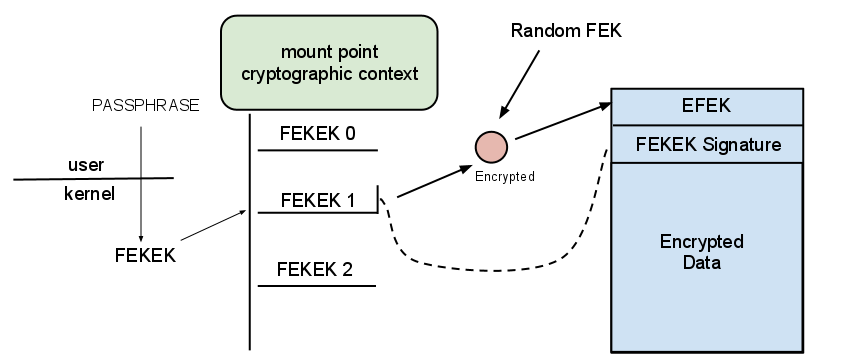
\includegraphics[scale=0.4]{eCryptfsNormalOperation.png} \end{center}
\caption{eCryptfs normal key operation} \label{fig:ecryptfsnormal} \end{figure}

\section{eCryptfs boundary mode}
\label{sec:boundarymode}
The modifications to eCryptfs presented in this chapter are inspired by the work of Leo Dorrendorf on increasing the resilience of
encrypted file systems to memory-based attacks \cite{Dorrendorf2011}. The keying method of eCryptfs has been modified to add a
notion of security boundaries between different parts of the file system, toward the end of providing a usable mobile device even
while portions of the file system cannot be accessed. In the traditional keying mode for eCryptfs, the master key is
F(EK)$^{2}$, and it must always remain memory resident, for if it is removed then no files can be accessed whatsoever.
Any device would quickly cease to operate in such a situation. A third, interstitial tier of keys, here called ``boundary'' keys, has
been introduced. When the device is locked, this key tier allows the master key to be removed from memory, along with any unnecessary
boundary keys, leaving accessible only the portion of the file system necessary to keep the device operational.

The question of where to draw boundaries immediately arises. The Android security architecture is designed, first and foremost,
around ``sandboxing'' applications . From a storage perspective, this means that applications are not allowed to access either
system data or data associated with other applications. The official documentation on security and permissions describes it this way: 
\begin{quote} 
A central design point of the Android security architecture is that no application, by default, has permission to perform any
operations that would adversely impact other applications, the operating system, or the user.  This includes reading or writing the
user's private data (such as contacts or e-mails), reading or writing another application's files, performing network access,
keeping the device awake, etc. \cite{securitydoc} 
\end{quote} 
It therefore seems natural to reinforce the security
mechanisms already in place with cryptographic boundaries.  One detail of the Android security architecture is particularly useful
for this purpose: 
\begin{quote} 
At install time, Android gives each package a distinct Linux user ID. The identity remains constant
for the duration of the package's life on that device. On a different device, the same package may have a different UID; what
matters is that each package has a distinct user ID (UID) on a given device. \cite{securitydoc}
\end{quote} 
This UID is used to establish file ownership for applications, which is convenient because it means that each UID can be associated
with a boundary key.  If that boundary key is removed from memory along with the master key, then even an attacker who has access to
the running device will not be able to decrypt the data associated with that application.

Boundary keys are generated by concatenating the master key with the UID of the file, and then hashing the result.  Boundary keys
are used as F(EK)$^{2}$, and the master key generated from the user's passphrase becomes F(EK)$^{3}$. Currently
only 128 bit keys hashed with MD5 are supported because that was the most accessible key length and algorithm already available
within eCryptfs, but it would not be a significant amount of work to expand the supported set of key sizes and hash algorithms. As
seen in Figure \ref{fig:ecryptfsboundary}, a list of boundary keys is kept alongside the list of master keys (internally referred
to as global authentication tokens).  When a file is opened, the boundary key for the relevant UID is retrieved. If the boundary key
cannot be located, but the master key is available, then the boundary key is derived from the master. This derivation is performed
when an application is opened for the first time after the device has been unlocked.

\begin{figure}[!htb] 
\begin{center}
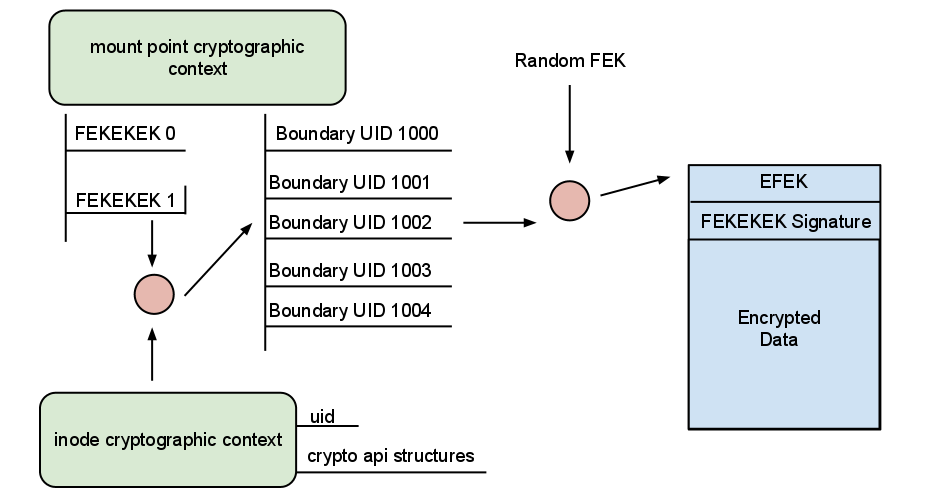
\includegraphics[scale=0.4]{eCryptfsBoundaryMode.png}\end{center}
\caption{eCryptfs Boundary Mode} \label{fig:ecryptfsboundary} \end{figure}

\section{Supporting eCryptfs Boundaries in Android}

\subsection{The Android Boot Process} How eCryptfs might be integrated into the Android platform cannot be understood without first
taking a quick look at the internals of the Android boot process. During startup, the ``bootloader'' is the first piece of code to
execute that is not hardwired into a device. Unlike a desktop Linux system, where open-source bootloaders such as GRUB are used,
phone manufacturers typically use proprietary bootloaders. While the sources for these bootloaders are not open to inspection, the
principles they operate on are well known. The bootloader, for at least the Nexus series of devices, can be interacted with via the
\texttt{fastboot} protocol. The Android Open Source Project includes the source for the \texttt{fastboot} utility, which can be used
to unlock the bootloader, flash images, and perform other functions that only the bootloader can do.  During normal startup the
primary task of the bootloader is to load the Android kernel into memory and pass control of the system over to it. 

The Android kernel will initialize the hardware and prepare the device itself for use. On an Android device, the \texttt{boot}
partition is separated from the \texttt{system} and \texttt{userdata} partitions (see chapter \ref{ch:forensics}). The boot
partition contains the kernel and a ``ramdisk.''  The ramdisk is a small file system that contains the core binaries and
configuration files needed to start the system. In most Linux-based systems, Android included, \texttt{init} is the ``grandmother''
of all processes. Everything outside of the kernel is launched by \texttt{init} directly or by a process that was
previously started by \texttt{init} \cite{eneaboot}. The Android \texttt{init} process is specialized for Android and does not coincide with
\texttt{init} as it is implemented on any other Linux distribution, thus hereafter \texttt{init} refers to \texttt{init} as it is
implemented in Android.  The configuration for \texttt{init} is held in two files on the ramdisk, \texttt{init.rc} and
\texttt{init.PRODUCTNAME.rc} where \texttt{PRODUCTNAME} is the internal name for the board on the device. The Nexus S, for example, is termed
``Herring,'' so \texttt{init} looks at \texttt{init.rc} and \texttt{init.herring.rc}.\footnote{A note on naming: the device and the
board for the device are named separately, but necessarily correlate. So, the Nexus One has a device name of ``passion,'' but a
board/kernel name of ``mahimahi.'' The Nexus S has a device name of ``crespo'' or ``crespo4g,'' depending on whether it is a Nexus S
or a Nexus S 4G, but they both have a board/kernel name of ``Herring.''} These configuration files are written in a script syntax
specific to \texttt{init} that supports basic functions which should be familiar, such as \texttt{mount}, \texttt{chmod}, and
\texttt{chown}, as well as more advanced functionality such as triggers based upon system properties.  Triggers in \texttt{init}
will be examined more thoroughly in section \ref{ssec:encryptionboot}. These scripts set up the file system layout of the device and
start all of the system services that make up Android as the user knows it. A typical line in an \texttt{init} script might look
like Table \ref{tab:initmount} which tells \texttt{init} to mount the \texttt{system} partition with the mount flags \texttt{wait}, and the mount
options \texttt{ro}. This is very similar to a standard mount command from a shell, but the syntax is slightly different. This will
be translated by \texttt{init} into an actual mount call to the kernel. 
\begin{table}[!htb]
\lstinputlisting{tables/init-mount}
\caption{Mounting a file system from within init.herring.rc}
\label{tab:initmount}
\end{table}


\subsection{Booting an Encrypted Device} \label{ssec:encryptionboot}

As described in the documentation for the implementation of encryption in Honeycomb\footnote{Honeycomb was the release of Android
immediately preceding Ice Cream Sandwich, and available for tablets only. There is no official documentation for the encryption
mechanism of Ice Cream Sandwich, but it functions as described in the Honeycomb document.} \cite{honeycombcrypt}, most of the heavy
lifting related to handling encrypted devices is performed by \texttt{vold}, the Android volume daemon. The volume daemon is the
system service responsible for keeping track of storage on an Android device. The primary mechanism for \texttt{init} to communicate
with the outside world, including \texttt{vold}, is the notion of a \emph{system property}.  Android has an elaborate property system
which is outside the scope of this discussion, but essentially \texttt{init} maintains a shared memory region where properties can
be set and retrieved. This shared region is visible to every process on the system \cite{propertysystem}. These ``native'' system
properties are distinct from system properties in Java, though native system properties are available to Java code via
JNI\footnote{JNI is the ``Java Native Interface,'' which is used to execute native code, typically C++, from within Java. Android
makes extensive use of JNI.}. The Honeycomb implementation document describes how these properties are used during boot with an
encrypted device:

\begin{quote} When init fails to mount /data, it assumes the file system is encrypted, and sets several properties: ro.crypto.state =
``encrypted" vold.decrypt = 1. It then mounts /data on a tmpfs ramdisk, using parameters it picks up from ro.crypto.tmpfs\_options,
which is set in init.rc.  \ldots The framework starts up, and sees that vold.decrypt is set to ``1". This tells the framework that it
is booting on a tmpfs /data disk, and it needs to get the user password. First, however, it needs to make sure that the disk was
properly encrypted. It sends the command ``cryptfs cryptocomplete" to vold, and vold returns 0 if encryption was completed
successfully, or -1 on internal error, or -2 if encryption was not completed successfully. \cite{honeycombcrypt}
\end{quote}

To summarize, \texttt{init} always attempts to mount \texttt{/data} as if it were unencrypted. This fails if the device is
encrypted, and then sets the appropriate system properties to denote the results of the attempted mount. When the framework starts,
\texttt{init} reads those properties, and calls \texttt{vold} if necessary. When called upon, it is the responsibility of
\texttt{vold} to handle setup for the \texttt{dm-crypt} device, making sure it gets decrypted and mounted at \texttt{/data}, while it
is the responsibility of the minimal framework to accept a password from the user and pass it to \texttt{vold}. Once \texttt{/data}
is successfully mounted, the rest of the framework services are started and the system is ready for use.

\subsection{Supporting eCryptfs in \texttt{vold}} \label{sec:ecryptfsvold} Just as the brains for handling \texttt{dm-crypt} were
placed in \texttt{vold} by Google, here all of the support for handling eCryptfs volumes is also placed in \texttt{vold}. Normally,
eCryptfs ships with a fully developed set of user space utilities to help with key and volume management. Rather than cross-compiling
the full set of utilities, the decision was made by the author to build only a minimal set of eCryptfs user space functionality into
an external library, available in the source tree accompanying this paper at \texttt{external/libecryptfs}.  The eCryptfs code was
mostly kept intact, with the exception of the hash function. The stock utilities use Mozilla's \texttt{libnss} to perform the
necessary hashes, but Android does not have \texttt{libnss} and cross-compilation is non-trivial. Android does, however, ship with
the OpenSSL crypto libraries, which include a full set of hash functions. Those functions were used in lieu of \texttt{libnss}.
Additionally, Android does not ship with keyutils, which is the user space library for interacting with the kernel key retention
service.  This library is required by \texttt{libecryptfs} to insert the key into the kernel. The keyutils library is included in
the source tree accompanying this paper at \texttt{external/libkeyutils}. 

Normally, if an eCryptfs volume is mounted by hand, a user generates a key from a passphrase and adds it to a keyring in the kernel
by using \texttt{ecryptfs-add-passphrase}.  This key is used as the master key for the eCryptfs volume. On Android the same
procedure is followed, but \texttt{vold} replaces \texttt{ecryptfs-add-passphrase}, and the signature of the key is recorded in the
system property \texttt{vold.ecryptfs\_options}, which actually contains the literal mount options required to mount an eCryptfs
volume on the device. Table \ref{tab:generate-key} shows the actual code in \texttt{vold} which calls \texttt{libecryptfs} to insert
the key into the kernel. 

\begin{table}[!htb]
\lstinputlisting{tables/generate-key} 
\caption{Function added to vold for eCryptfs key generation}
\label{tab:generate-key}
\end{table}

The \texttt{vold} function \texttt{cryptfs\_check\_passwd}, which is used to verify that a password is correct for mounting an
encrypted volume, has been modified to include a call to the new \texttt{cryptfs\_generate\_ecryptfs\_key}. Thus, when a user enters
their password to decrypt the device at boot, the corresponding eCryptfs mount key is inserted into the keyring at the same time.

The Android kernel must also support eCryptfs and key retention, which the default Android kernel does not. Enabling support for
these options is easy, however, as it simply involves enabling the appropriate options in the kernel configuration, building the
kernel, and placing it into the appropriate device folder within the Android Open Source Project, prior to building. The code for
this paper includes the modified kernel source in the \texttt{kernel} subdirectory, and the compiled kernel can be found in
\texttt{device/samsung/crespo} (crespo because a Nexus S was used for testing).

\subsection{Enabling eCryptfs Encryption} Normally, an Android 4.0 device is encrypted in-place, that is the existing data is
encrypted without being moved, but this is a difficult operation with eCryptfs. In-place encryption is a relatively easy operation
with block level encryption, as the device can be unmounted and each block encrypted where it lies. On the other hand, a multitude
of problems present themselves when the issue of encrypting existing data files with eCryptfs is contemplated.  The typical process
for encrypting existing files with eCryptfs is to create an empty eCryptfs mount and then copy the existing files to the eCryptfs
file system.  This could be done, but it would come with the requirement that no more than half the data partition be in use prior to
encryption. Even if that constraint were accepted, Android does not include a native file copy utility.\footnote{Although Android
\texttt{init} does have a file copy, it is quite rudimentary and would not suffice for the purpose at hand.} Copy functionality
could be written, of course, but a robust file copy is not as simple as it may seem. Instead of reinventing the wheel, a third-party
shell such as Busybox could be included in the system build, but then core OS functions are relying on shell scripts. In short,
encrypting existing files with eCryptfs on Android is possible, but appeared to be more trouble than it was worth.

There is a way to avoid the in-place encryption problem, however. When a device is encrypted, the command ``cryptfs enablecrypto
inplace'' is sent to \texttt{vold}, which instructs it to perform an in-place encryption of the \texttt{userdata} partition. Yet
\texttt{vold} also supports the command ``cryptfs enablecrypto wipe,'' though is not enabled in the official Android release. The
Android mount service, which is the Java service that makes the call to \texttt{vold}, can be easily modified to send the ``wipe''
incantation instead of ``inplace.'' It is important to note that this does not securely wipe the device. It merely recreates the
file system. Any data that existed prior to encrypting the device should be treated, for forensics purposes, as if it still exists.
Mooreover, the entire data partition is not encrypted with eCryptfs. Only \texttt{/data/data} is encrypted, as a demonstration. This
includes all of the application data on the phone, but certainly not all of the available forensic artifacts.

For the phone to boot after \texttt{/data/data} has been encrypted, \texttt{init} needs to be instructed to mount
\texttt{/data/data} as an eCryptfs volume. This can be done with one line in \texttt{init.rc} at the end of the
\texttt{post-fs-data} section. The \texttt{post-fs-data} section is executed as a trigger by \texttt{init}. Triggers in
\texttt{init} respond to system properties being set to a certain value. When an encrypted phone boots, after \texttt{vold} has
successfully mounted the encrypted partition and the master key has been inserted into the keyring, the system property
\texttt{vold.decrypt} is set to the value \texttt{trigger\_post\_fs\_data}. The act of setting this property signals to
\texttt{init} that the \texttt{post-fs-data} section of \texttt{init.rc} should be run. Triggers are easy to implement, and this one
is shown in Table \ref{tab:post-fs-data-trigger}.  
\begin{table}[!htb] 
\lstinputlisting{tables/post-fs-data-trigger} 
\caption{Trigger in init to setup decrypted data partition}
\label{tab:post-fs-data-trigger} 
\end{table} 
An attempt is made every boot to mount
\texttt{/data/data} as an eCryptfs volume, and if the volume is not encrypted it will silently fail. 

A final modification was necessary to correctly retrieve the mount options for mounting the eCryptfs volume. Retrieving these
options is complicated by the fact that eCryptfs expects the key signature of the master key to be passed as a mount option.
Including this kind of dynamic behavior would be difficult in \texttt{init.rc}, so it was placed in \texttt{init} proper. This is
the reason why \texttt{cryptfs\_generate\_ecryptfs\_key} stored the necessary mount options in a system property, as discussed in
section \ref{sec:ecryptfsvold}. The mount function in \texttt{init} has been modified to read the mount options from this system
property if the file system type is ``ecryptfs,'' as shown in Table \ref{tab:init-ecryptfs-mount}.

\begin{table}[!htb] 
\lstinputlisting{tables/init-ecryptfs-mount}
\caption{Reading eCryptfs mount options from system property} 
\label{tab:init-ecryptfs-mount}
\end{table}

\section{Removing Keys}

Encrypting the data partition of a device with separate keys for each application serves little purpose if the
boundary keys are not removed when the device is locked. This section describes how pressing the power button on a device can
trigger the removal of the master key and any specified boundary keys. This demonstration does not sufficiently sanitize freed
memory to completely prevent key extraction through live analysis (see chapter \ref{ch:future} for more details).

\subsection{Messaging in eCryptfs}
 
There is a messaging system built into eCryptfs for handling communication between user space and kernel space. Normally, eCryptfs
supports running a daemon called \texttt{ecryptfsd} that can be called upon to perform tasks outside of the kernel.  Typically,
\texttt{ecryptfsd} is used for an entirely different keying mode, where eCryptfs volumes are encrypted with a public key and
decrypted with a private key.  In this keying mode, when an encrypted file is opened eCryptfs reads a public key out of the file
header, instead of an EFEK, and then calls out to \texttt{ecryptfsd} to retrieve the corresponding private key material \cite{ecryptfspki}. More
generally, \texttt{ecryptfsd} provides a way for the keying mechanism of eCryptfs to be extended.  Chapter \ref{ch:future} includes
a discussion of how boundary keys might be re-implemented using \texttt{ecryptfsd}, affording a considerable increase in
flexibility.

Messaging within eCryptfs works by reading and writing messages to the device handle \texttt{/dev/ecryptfs}, which is registered as
a ``miscellaneous'' device. A miscellaneous device is a small driver implemented to support a special purpose not general enough to
warrant a new device class in the kernel. In this case the purpose is communication with \texttt{ecryptfsd}.\footnote{Previously,
\texttt{NETLINK} messages were used, which is a socket-like mechanism for communication with the kernel, but that method has lost
favor within eCryptfs.} As the current implementation of boundary keys does not rely on calling out to \texttt{ecryptfsd} for key
computation, running \texttt{ecryptfsd} is not necessary, and the messaging system can still be used by writing to
\texttt{/dev/ecryptfs} directly. 

Three new messages have been defined: \texttt{ECRYPTFS\_MSG\_CLEARMASTER}, \texttt{ECRYPTFS\_MSG\_CLEARBOUNDARY}, and
\texttt{ECRYPTFS\_MSG\_REGMASTER}, hereafter referred to as \texttt{clearmaster}, \texttt{clearboundary}, and \texttt{regmaster},
respectively. The payload of a \texttt{clearmaster} message must be the path to the mount point for which the master key should be
cleared, as each mounted eCryptfs file system is keyed independently. When \texttt{clearmaster} is received by the kernel, all
references to the master key - F(EK)$^{3}$ - within the kernel are removed from memory. This will \emph{not} remove the
actual key from the user's keyring. It is the responsibility of user space to remove the key from the keyring, which in the Android
implementation is handled by \texttt{vold}.  Technically, what \texttt{clearmaster} does is ``walk'' the list of global
authentication tokens associated with a given mount point, zero them all with \texttt{memset}, and remove them from the list.  At
this point the key itself must be removed from the user's keyring or all files will remain decryptable. One \texttt{clearboundary}
message for each boundary key being cleared should be sent after the master key has been cleared. If the boundary keys are cleared
prior to clearing the master key, then it is possible the boundary keys could be recalculated for a given UID. The
\texttt{clearboundary} message payload should start with four bytes specifying the UID of the boundary to clear, immediately
followed by a string specifying the mount point of the eCryptfs file system. Boundary keys are cleared in a fashion similar to master
keys: the list associated with the mount point is walked, each structure is zeroed, and the items removed.  No boundary keys are
held in user space memory, so they have actually been removed as soon as the message is sent to the kernel. 

In order for key removal to function properly, it was necessary to force eCryptfs to recalculate the cryptographic context for
each file as it is opened, which does have some impact on performance. Normally the FEK is stored in a lookaside cache after the
file is opened, but that allows access to the file even after the master and boundary keys have been cleared. The \texttt{release}
function in eCryptfs has been modified to remove the FEK from cache upon file close.


Within Android, these messages are sent by \texttt{vold}, relying on the same stripped-down \texttt{libecryptfs} mentioned
previously.  A set of new functions has been defined in \texttt{vold} that receive messages from the Java-based mount service and
relay them to the kernel. These functions, in turn, are exposed as \texttt{vold} commands that are accessible from the Android
framework. Any application with permission to control \texttt{vold} can clear or re-register keys by executing one of the following
commands: \texttt{cryptfs clearmaster}, \texttt{cryptfs clearboundary <uid>}, or \texttt{cryptfs regmaster}. Note that while the
kernel messages require a mount point to be passed, the \texttt{vold} commands do not. This implementation assumes that
\texttt{/data/data} is the only mounted eCryptfs volume. It would be easy to extend the \texttt{vold} commands to support
multiple encrypted volumes. Additionally, the \texttt{clearmaster} command in \texttt{vold} unlinks the master key from the
user space keyring
handled by the kernel key retention service, which contains the actual private key material for the eCryptfs mount. This key
material was originally generated from the unlock passphrase and stored in the keyring by \texttt{vold}.

When an Android device goes to sleep, either because the user pressed the power button or because the inactivity timeout was
triggered, the \texttt{ACTION\_SCREEN\_OFF} intent\footnote{Intents are messages within the Android framework. See
\texttt{developer.android.com} for details.} is broadcast. Any listeners that have registered to receive this intent are notified.
In order to accommodate boundary key removal, the mount service has been registered to receive this intent and calls \texttt{cryptfs
clearmaster} along with \texttt{cryptfs clearboundary} when the intent is received. 

Finally, any application that is having its boundary key cleared is stopped. This stands in contrast to the normal behavior
of simply pausing applications when the phone is locked. An application remains memory resident when it has its activities paused.
If a paused application is resumed without ever being completely killed, any data in memory is still available, even if the boundary key
has been removed. Killing applications during the lock process, rather than merely pausing them, ensures that they must
read data back off of disk. If the boundary key has been removed, disk reads will fail. Whether or not the application will
transparently return to its previous state when reopened depends on how gracefully the application handles being terminated. 

For demonstration purposes, the \texttt{clearboundary} call available in the code accompanying this paper has hard-coded the UID of
the application to secure during device lock. A hard-coded UID is not terribly useful, but serves as a placeholder where custom
logic could be added to determine what applications have data that should be protected, as seen in Table \ref{tab:mountservice}.
Ideally, the list would be accessible through a configuration interface presented to the user.

\begin{table}[!htb]
\lstinputlisting{tables/mountservice.java}
\caption{Clearing keys from the mount service}
\label{tab:mountservice}
\end{table}

When a device is unlocked, the master key for the volume is recalculated, inserted into the key retention service, and registered
as a global authentication token with eCryptfs by sending a \texttt{regmaster} message to the kernel module, with the signature of
the key that needs to be registered. 

\subsection{Alice Sends Bob Flowers}
\label{sec:alicebob}
The whole thing is complex, to be sure. A short, hypothetical example may help illustrate the purpose and process of eCryptfs boundary mode.  

Alice would like to send Bob some flowers. Unfortunately, flowers have been recently outlawed, along with all other outward displays
of affection. A busy woman, Alice tends to make lists for herself so that she does not forget important things, like sending Bob
flowers. She is heavily invested in \emph{ColorNote}, a note-taking application, which does offer password protection and encrypted
backups, but does not encrypt notes on the device. A closed source application, encryption cannot be added without considerable
effort. Alice is worried that her phone will be taken, her to-do list will be discovered, and that she will be locked away when the
government sees that she has been buying flowers. This fear was stoked by a document recently uncovered with a Freedom of
Information Act request, revealing that at least one government was looking at to-do lists during mobile seizures, as shown in
Figure \ref{fig:dhs} \cite{dhsfoia}. Alice wants to prevent someone with physical access to her device, should it be confiscated,
from seeing the contents of her to-do list. Android 4.x would protect her to-do list if the phone was captured while powered off, but
it has been rumored the government is hoarding OS exploits against phones, among other things. If the government can bypass the lock
screen on her phone, then it is all over for the poor lady. Alice would like to protect her to-do list even in the event that her
phone is seized and the lock screen can be bypassed, so that a ``logical acquisition,'' in forensics parlance, would be fruitless.
What is Alice to do?

\begin{figure}[!htb]
\begin{center}
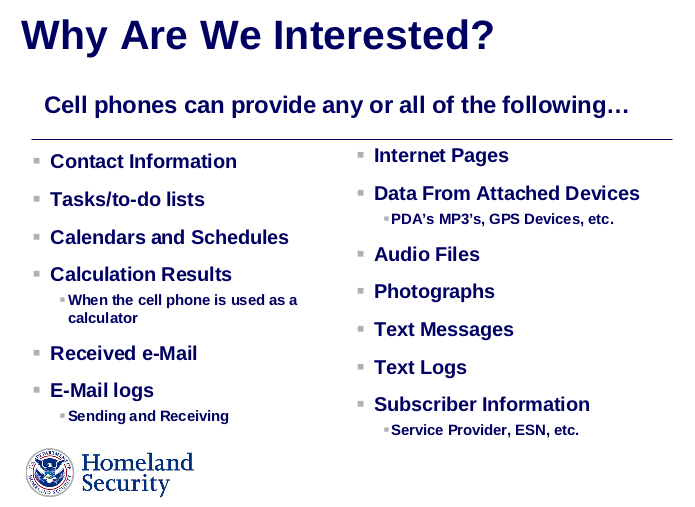
\includegraphics[scale=0.5]{dhs.png}
\end{center}
\caption{DHS mobile forensics training} 
\label{fig:dhs}
\end{figure}

Alice begins running an Android distribution that supports eCryptfs boundary mode. She configures the device such that the boundary
key for ColorNote is cleared every time the phone is locked or goes to to sleep. When she is using the phone, her private to-do list
is easily accessible. After the keys have been removed, the application fails to start entirely unless the phone has been properly
unlocked. Attempting to access the databases through \texttt{adb} simply returns \texttt{I/O error}. While this does not, by any
means, provide perfect security, Alice has forced the issue out of the realm of traditional post-mortem forensics. If an attacker
wanted to recover the data, either live memory analysis would need to be performed, or an out-of-band attack executed. The
passphrase might be determined from the smudge patterns on the screen, or the key simply extracted from Alice directly through a
rubber-hose attack. Neither the acquisition process described in chapter \ref{ch:forensics} nor inspection of the device from the
user interface as it is running will compromise Alice's data.
